The motion control is meant to give the robot a smooth and accurate movement that enables wall following and movement through most environments that could appear with the given constraints on the environment.

\subsection{Motor control}

The low level control is performed by the motor control. It receives a velocity message (right speed and left speed) and tries to keep the reference speeds by feeding them into two controllers, one for each wheel. The controllers takes the error (reference speed minus actual speed) and multiplies it with a constant that is tuned manually to obtain a good control performance. This type of controller is called a P-controller (P for proportional). The actual speed is calculated from the time derivative of the wheel encoder measurements and then subtracted from the reference speed to get the error.
With a steady speed the robot can be assumed to either move in a straight line or rotate on the spot depending on the reference signal.

\subsection{Angular and linear movement }

The two basic movements that are needed to explore the whole environment are rotation on the spot and moving straight. Rotation is performed by a P-controller that computes a control signal based on the difference between the reference angle and the actual angle. The angular speed is also saturated to prevent unreasonable high or low speeds. Further, the motion is smoothed by applying an acceleration phase while starting a rotation movement and a lower acceleration results in less wheel slippage and thereby a more accurate final angle. The output (rotation speed) from the rotation function is sent to one motor, and the other gets the rotation speed with switched sign. The architecture of the control system for rotation is shown in figure \ref{fig:rotation_blockdiagram}.

\begin{figure}[h]
\label{fig:rotation_blockdiagram}
    \begin{centering}
   	 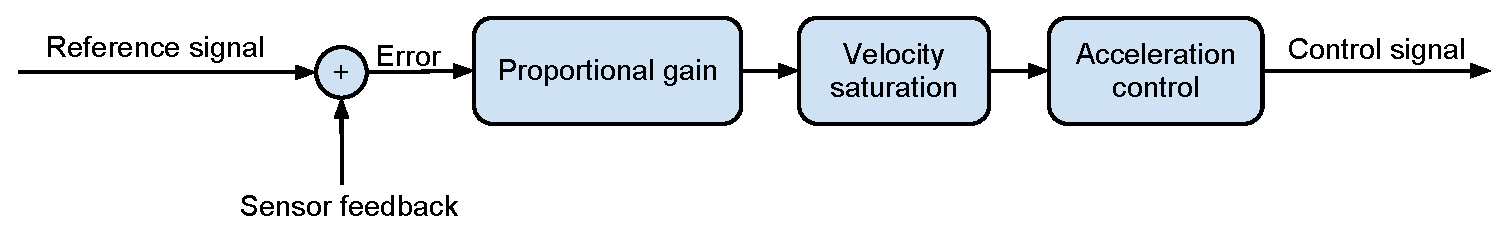
\includegraphics[scale=0.5]{figures/rotate_blockdiagram.pdf}
   	 \caption{Controller architecture for rotate function.}\label{fig:rotation_blockdiagram}
    \end{centering}
\end{figure}

The straight movement is based on the same idea but instead of sending a positive speed on one wheel and a negative on the other, both speeds have the same sign to either move the robot backwards or forward. 

\subsection{Wall following}

Wall following moves the robot along a wall and makes it turn so that most situations can be handled. The wall following node is using the previously mentioned functionalities, linear movement and angular movement, to be able to follow the wall. In addition to the encoder measurements it now uses the IR sensors to determine the distance and an angle to the wall. These measurements have the benefit of having a absolute error compared to the encoder measurements that drifts over time and the error integrates and eventually becomes very large.
	The sensor input is sent to a P-controller that controls the angle to the wall, so that the robot drives parallel to the wall, this makes the robot move in a fairly straight line while doing wall following. The distance to the wall is only controlled in case the robot exceeds a threshold of being too close or too far from the wall. This makes the robot behave smoother and do less corrections to keep the right distance and will also improve the odometry since the robot will turn less.
	The wall following functionality is based on a state machine that changes state when the wall cannot be followed any more without further actions. The state machine is shown in figure  \ref{fig:followWallStates} and the states are designed to handle most tricky situations that can appear in the environment. Conditions used in the state machine are explained in table \ref{table:conditions}.

TODO table
Condition	Description
rF	Right front IR sensor sees a wall
rL	Right left IR sensor sees a wall
WF	Wall in front detected


\begin{figure}[h]
    \begin{centering}
   	 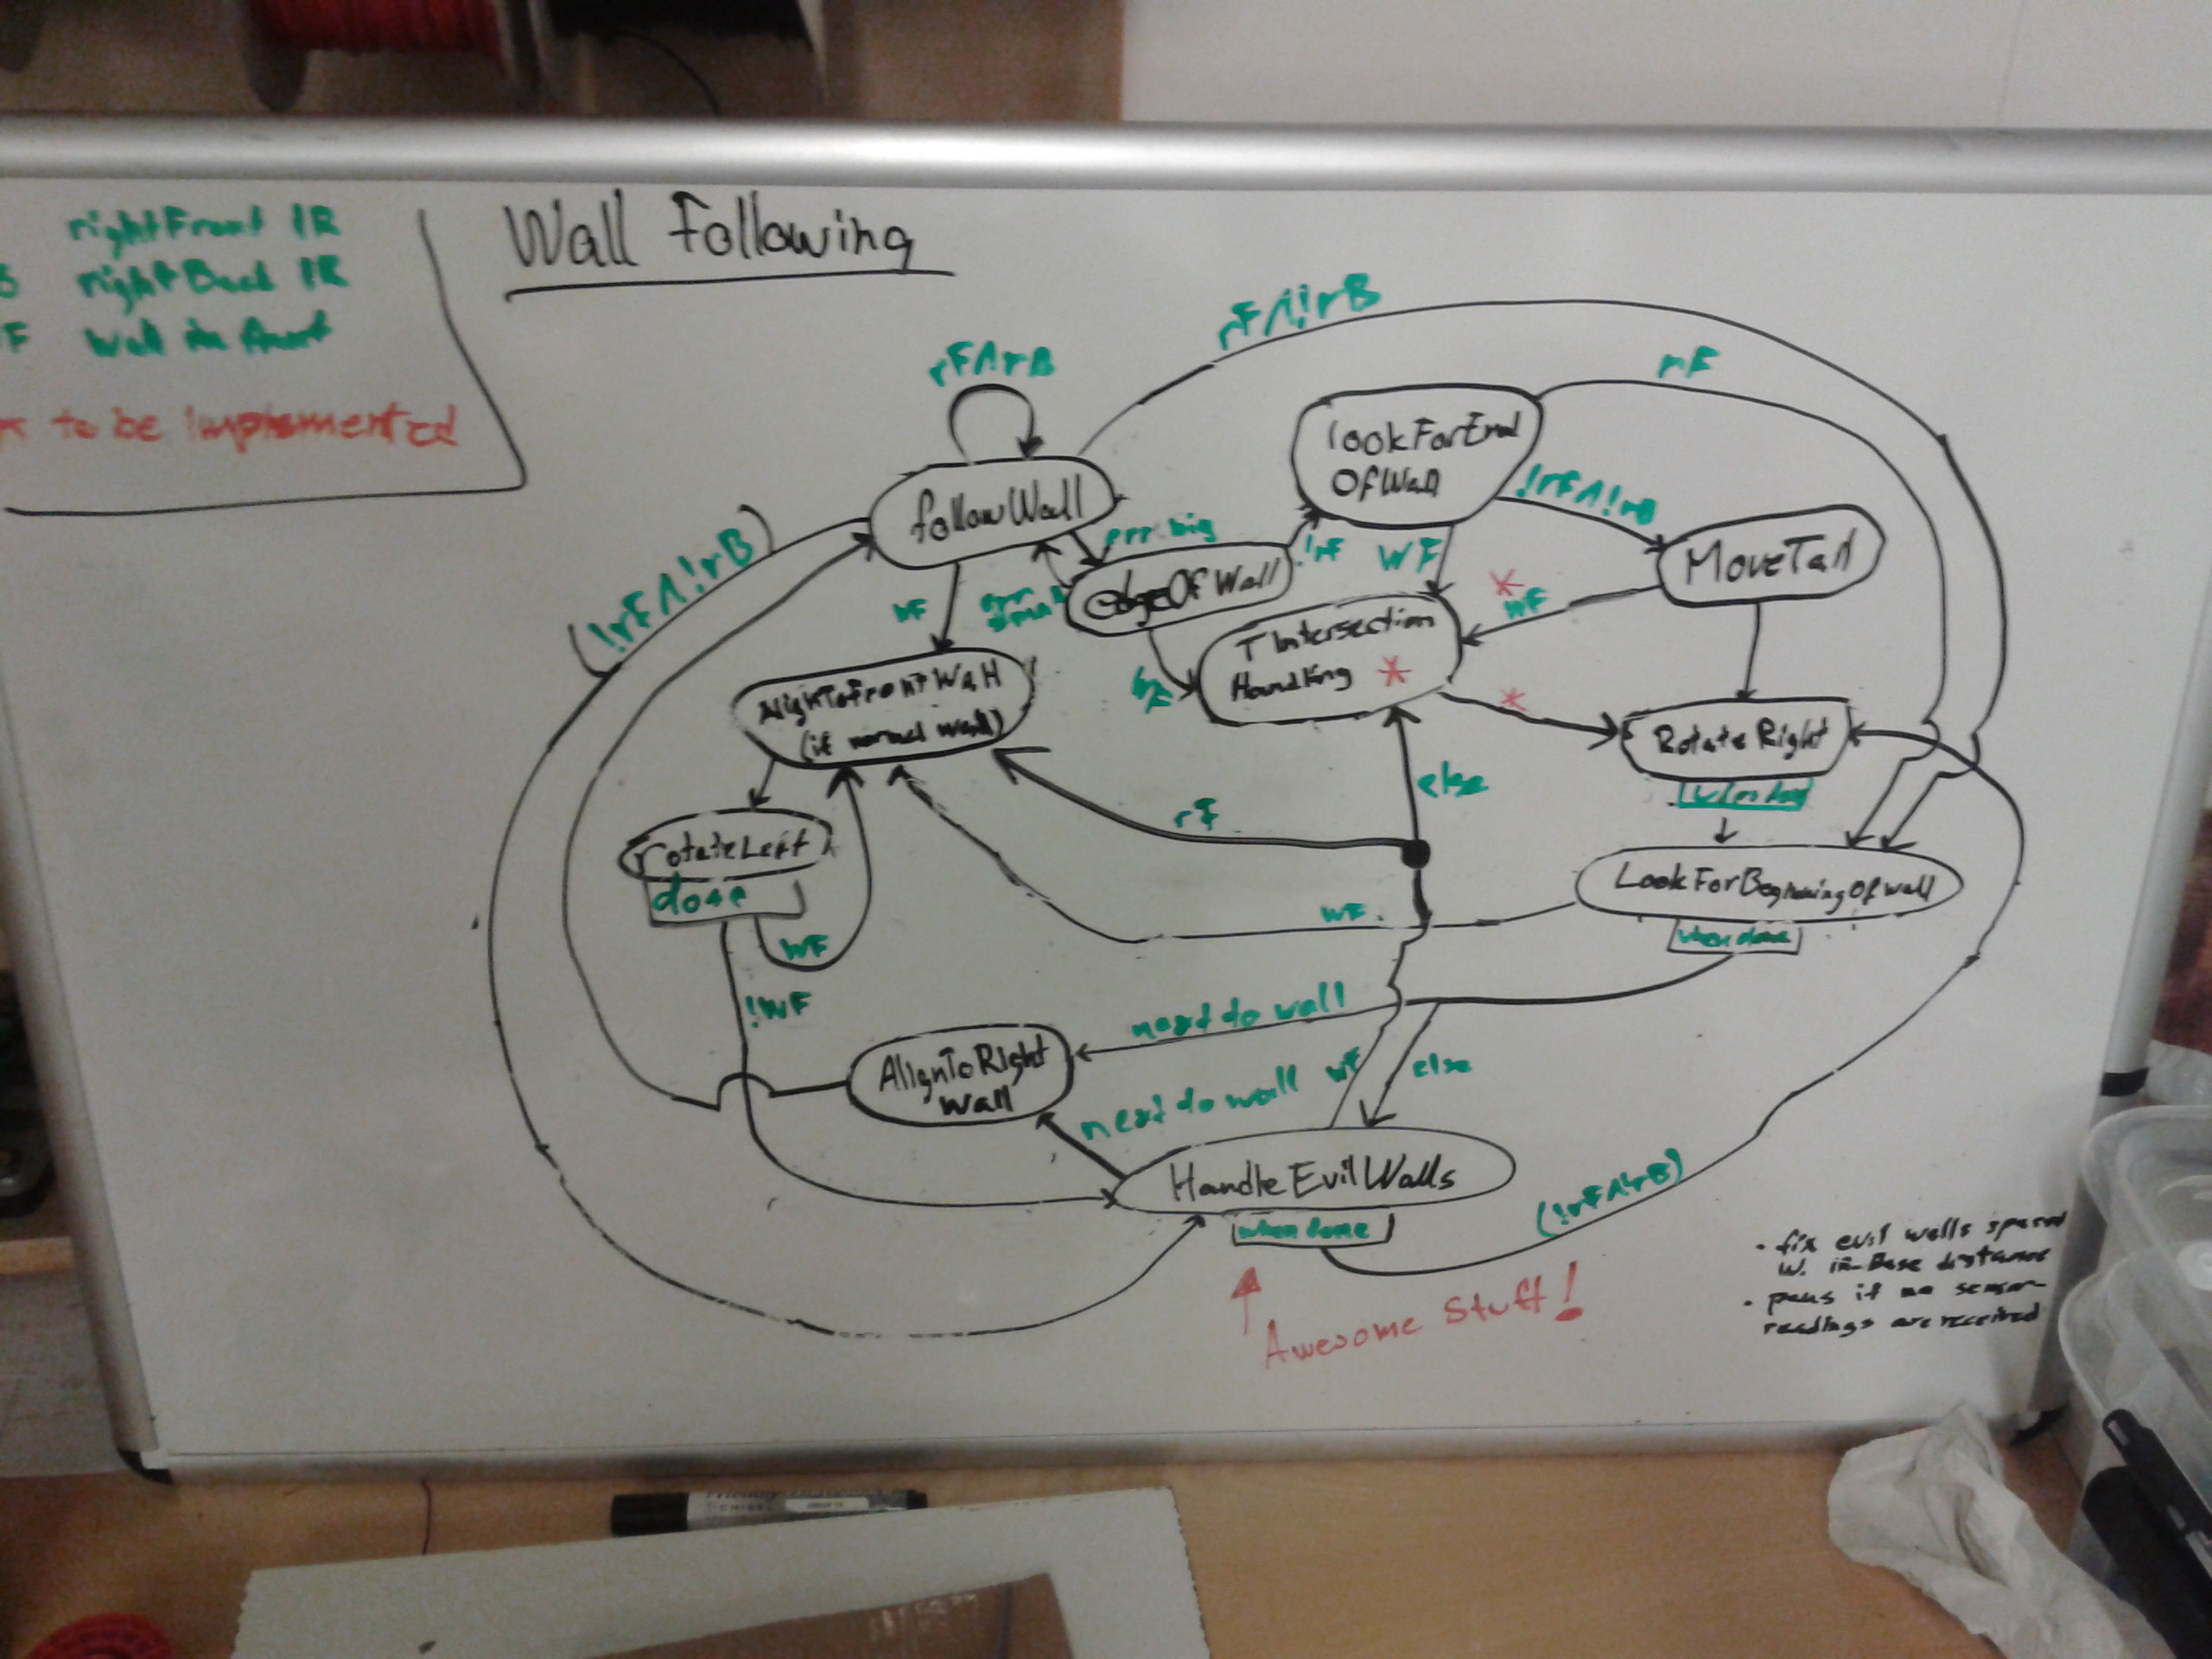
\includegraphics[scale=0.15]{figures/followWallStates.jpg}
   	 \caption{followWallStates, TODO: nice image.}\label{fig:followWallStates}
    \end{centering}
\end{figure}

The states are briefly explained in table \ref{table:followWallStates}. 
TODO table
State
Description
Follow Wall	A state that follows the right wall as long as there is a wall on the robot’s right side.
Rotate right	Rotates 90 degrees right.
Rotate left	Rotates 90 degrees left.
Align to wall	Aligns the robot to the right wall.
Align to front wall	Aligns the robot to the front wall.
Handle evil walls	If an end of a wall is detected in front, this state makes the robot turn left, go forward and turn right again to see if its possible to pass.
Move tail	If e.g. the right wall ends, this state moves the robot forward so that it has some clearance to to go around corners.
Edge of wall	This state prevents the robot form making quick heading corrections when a wall ends and the IR suddenly changes value.
Look for beginning of wall	If the robot starts to see a wall with the right front IR this state drives the robot straight forward until the right back IR sees the wall. 
Look for end of wall	If the robot is following a wall and the right front IR sensor doesn’t see the wall any more, this state is used to drive the robot straight forward until the right back IR doesn’t see the wall either.
T intersection handling	If the robot detects a wall in front, this state switches to rotate right state so that it checks if it’s possible to go right.

The following states handles most situations that could appear in the environment.

\subsection{Move to coordinate}

Sometimes it is necessary to move away from the wall in order to explore the whole environment. Move coordinate is used to do this, it’s based on the same basic functions as the wall following function is based on, namely the linear movement and the angular movement. As the name tells it moves to a specified coordinate by first rotating and then move straight to that point.

\subsection{Movement control}

Movement control uses all the functionality previously described here in section \ref{sect:motionControl} to be able to make any movement that is required, follow wall and move to coordinate, to explore the whole environment.